\section{Results}
\subsection{Results of the Theoretical Investigation}

\subsubsection{Sample Tables of Time vs. Lift Coefficient ($C_L$) for Bluff Body $n=2,\,6\,\text{and}\,12$}

\begin{table}[H]
	\centering
	\begin{tabular}{|c|c|}
		\hline
		\textbf{Time (s)} & \textbf{$C_L$} \\
		\hline
		$1 \times 10^{-5}$ & $2.0946206 \times 10^{-11}$ \\
		\hline
		$2 \times 10^{-5}$ & $-6.5426717 \times 10^{-12}$ \\
		\hline
		$3 \times 10^{-5}$ & $-7.3241302 \times 10^{-12}$ \\
		\hline
		$4 \times 10^{-5}$ & $-6.6677951 \times 10^{-12}$ \\
		\hline
		$5 \times 10^{-5}$ & $-5.1304516 \times 10^{-12}$ \\
		\hline
		$6 \times 10^{-5}$ & $-4.3635501 \times 10^{-12}$ \\
		\hline
		$7 \times 10^{-5}$ & $-3.6837751 \times 10^{-12}$ \\
		\hline
		$8 \times 10^{-5}$ & $-3.2635206 \times 10^{-12}$ \\
		\hline
		$9 \times 10^{-5}$ & $-2.8660898 \times 10^{-12}$ \\
		\hline
		$1.0 \times 10^{-4}$ & $-2.4321206 \times 10^{-12}$ \\
		\hline
		$1.1 \times 10^{-4}$ & $-2.1246574 \times 10^{-12}$ \\
		\hline
		$1.2 \times 10^{-4}$ & $-1.8807166 \times 10^{-12}$ \\
		\hline
		$1.3 \times 10^{-4}$ & $-1.6461582 \times 10^{-12}$ \\
		\hline
		$1.4 \times 10^{-4}$ & $-1.4100222 \times 10^{-12}$ \\
		\hline
		$1.5 \times 10^{-4}$ & $-1.1994923 \times 10^{-12}$ \\
		\hline
		$1.6 \times 10^{-4}$ & $-1.0306274 \times 10^{-12}$ \\
		\hline
		$1.7 \times 10^{-4}$ & $-8.6746456 \times 10^{-13}$ \\
		\hline
		$1.8 \times 10^{-4}$ & $-7.3730846 \times 10^{-13}$ \\
		\hline
		$1.9 \times 10^{-4}$ & $-6.2413158 \times 10^{-13}$ \\
		\hline
		$2.0 \times 10^{-4}$ & $-5.1195718 \times 10^{-13}$ \\
		\hline
	\end{tabular}
	\label{tab:1FaceClTable}
	\caption{Example of the first 20 values of the table produced by the simulation. Time vs. Lift Coefficient ($C_L$) for bluff body $n=2$}
\end{table}

\begin{table}[H]
	\centering
	\begin{tabular}{|c|c|}
		\hline
		\textbf{Time (s)} & \textbf{$C_L$} \\
		\hline
		$1 \times 10^{-5}$  & $-3.3657419 \times 10^{-12}$ \\
		\hline
		$2 \times 10^{-5}$  & $-1.9884762 \times 10^{-11}$ \\
		\hline
		$3 \times 10^{-5}$  & $-9.3048242 \times 10^{-12}$ \\
		\hline
		$4 \times 10^{-5}$  & $-4.4630770 \times 10^{-12}$ \\
		\hline
		$5 \times 10^{-5}$  & $-2.0927449 \times 10^{-12}$ \\
		\hline
		$6 \times 10^{-5}$  & $-7.7780466 \times 10^{-13}$ \\
		\hline
		$7 \times 10^{-5}$  & $-6.0321899 \times 10^{-14}$ \\
		\hline
		$8 \times 10^{-5}$  & $4.8061350 \times 10^{-13}$ \\
		\hline
		$9 \times 10^{-5}$  & $7.3193765 \times 10^{-13}$ \\
		\hline
		$1.0 \times 10^{-4}$ & $9.6907823 \times 10^{-13}$ \\
		\hline
		$1.1 \times 10^{-4}$ & $1.1376576 \times 10^{-12}$ \\
		\hline
		$1.2 \times 10^{-4}$ & $1.2174253 \times 10^{-12}$ \\
		\hline
		$1.3 \times 10^{-4}$ & $1.2584116 \times 10^{-12}$ \\
		\hline
		$1.4 \times 10^{-4}$ & $1.3129809 \times 10^{-12}$ \\
		\hline
		$1.5 \times 10^{-4}$ & $1.3234668 \times 10^{-12}$ \\
		\hline
		$1.6 \times 10^{-4}$ & $1.3258472 \times 10^{-12}$ \\
		\hline
		$1.7 \times 10^{-4}$ & $1.3305942 \times 10^{-12}$ \\
		\hline
		$1.8 \times 10^{-4}$ & $1.3123542 \times 10^{-12}$ \\
		\hline
		$1.9 \times 10^{-4}$ & $1.2928728 \times 10^{-12}$ \\
		\hline
		$2.0 \times 10^{-4}$ & $1.2666382 \times 10^{-12}$ \\
		\hline
	\end{tabular}
	\label{tab:6FaceClTable}
	\caption{Example of the first 20 values of the table produced by the simulation. Time vs. Lift Coefficient ($C_L$) for bluff body $n=6$}
\end{table}

\begin{table}[H]
	\centering
	\begin{tabular}{|c|c|}
		\hline
		\textbf{Time (s)} & \textbf{$C_L$} \\
		\hline
		$1 \times 10^{-5}$  & $-2.4598505 \times 10^{-11}$ \\
		\hline
		$2 \times 10^{-5}$  & $7.6579451 \times 10^{-12}$ \\
		\hline
		$3 \times 10^{-5}$  & $-2.1510813 \times 10^{-12}$ \\
		\hline
		$4 \times 10^{-5}$  & $-4.4206937 \times 10^{-12}$ \\
		\hline
		$5 \times 10^{-5}$  & $-2.2353308 \times 10^{-12}$ \\
		\hline
		$6 \times 10^{-5}$  & $-3.6197725 \times 10^{-12}$ \\
		\hline
		$7 \times 10^{-5}$  & $-2.8919916 \times 10^{-12}$ \\
		\hline
		$8 \times 10^{-5}$  & $-2.1972666 \times 10^{-12}$ \\
		\hline
		$9 \times 10^{-5}$  & $-1.6629472 \times 10^{-12}$ \\
		\hline
		$1.0 \times 10^{-4}$ & $-1.1636706 \times 10^{-12}$ \\
		\hline
		$1.1 \times 10^{-4}$ & $-7.5429574 \times 10^{-13}$ \\
		\hline
		$1.2 \times 10^{-4}$ & $-4.0834742 \times 10^{-13}$ \\
		\hline
		$1.3 \times 10^{-4}$ & $-1.3927346 \times 10^{-13}$ \\
		\hline
		$1.4 \times 10^{-4}$ & $2.5593892 \times 10^{-13}$ \\
		\hline
		$1.5 \times 10^{-4}$ & $4.2789616 \times 10^{-13}$ \\
		\hline
		$1.6 \times 10^{-4}$ & $6.3422462 \times 10^{-13}$ \\
		\hline
		$1.7 \times 10^{-4}$ & $5.5145736 \times 10^{-13}$ \\
		\hline
		$1.8 \times 10^{-4}$ & $6.3739292 \times 10^{-13}$ \\
		\hline
		$1.9 \times 10^{-4}$ & $6.7691966 \times 10^{-13}$ \\
		\hline
		$2.0 \times 10^{-4}$ & $7.1047796 \times 10^{-13}$ \\
		\hline
	\end{tabular}
	\label{tab:12FaceClTable}
	\caption{Example of the first 20 values of the table produced by the simulation. Time vs. Lift Coefficient ($C_L$) for bluff body $n=12$}
\end{table}

\subsubsection{Lift Coefficient ($C_L$) Over Time for each Bluff Body}
\label{sec:C_LvsTime}

\begin{figure}[H]
	\centering
	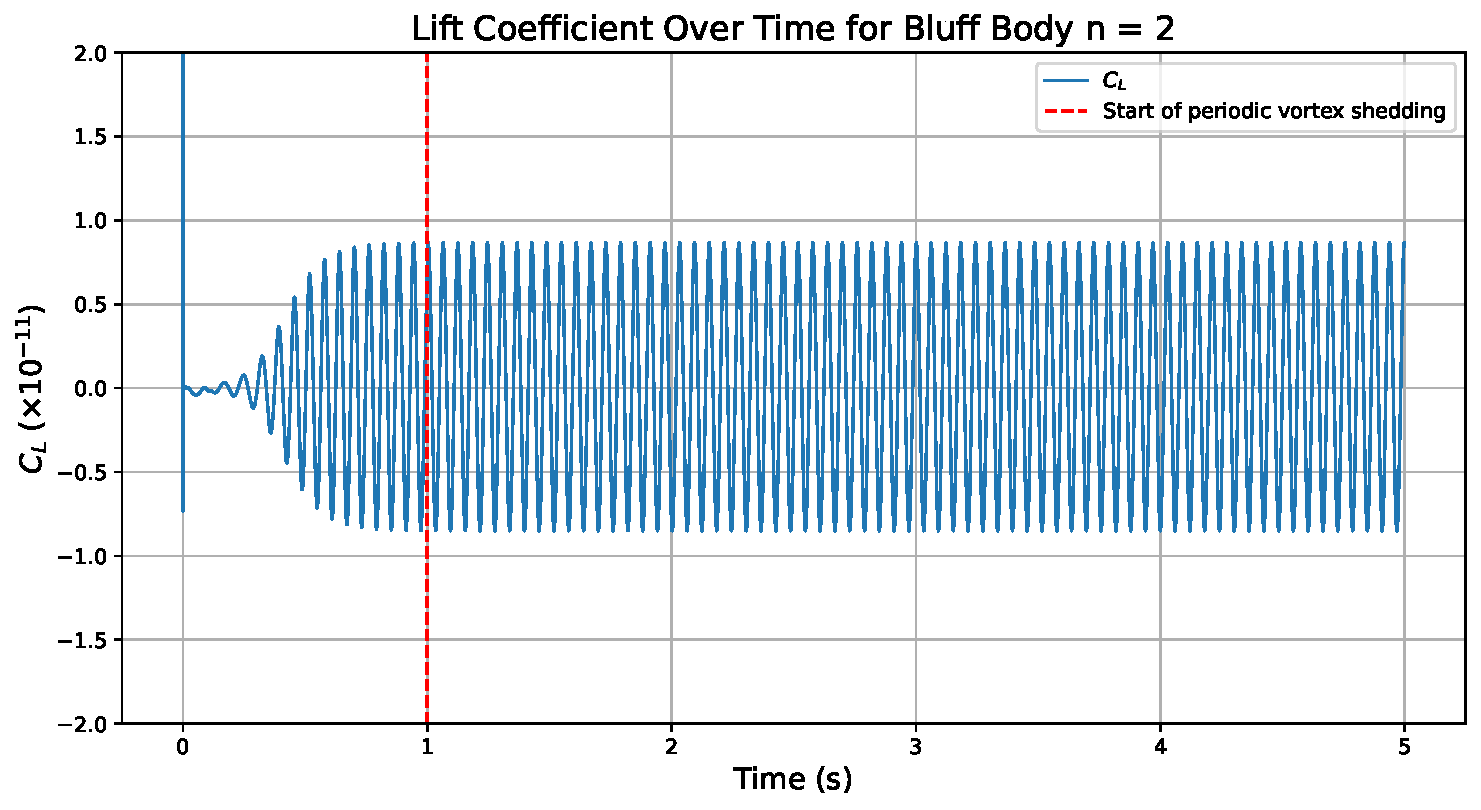
\includegraphics[width=\textwidth]{images/2face_graph}
	\caption{Lift coefficient $C_L$ over time for the bluff body $n=2$. The red dashed line indicates the start of periodic vortex shedding at $t = 1\,\mathrm{s}$.}
	\label{fig:2FaceGraph}
\end{figure}

\begin{figure}[H]
	\centering
	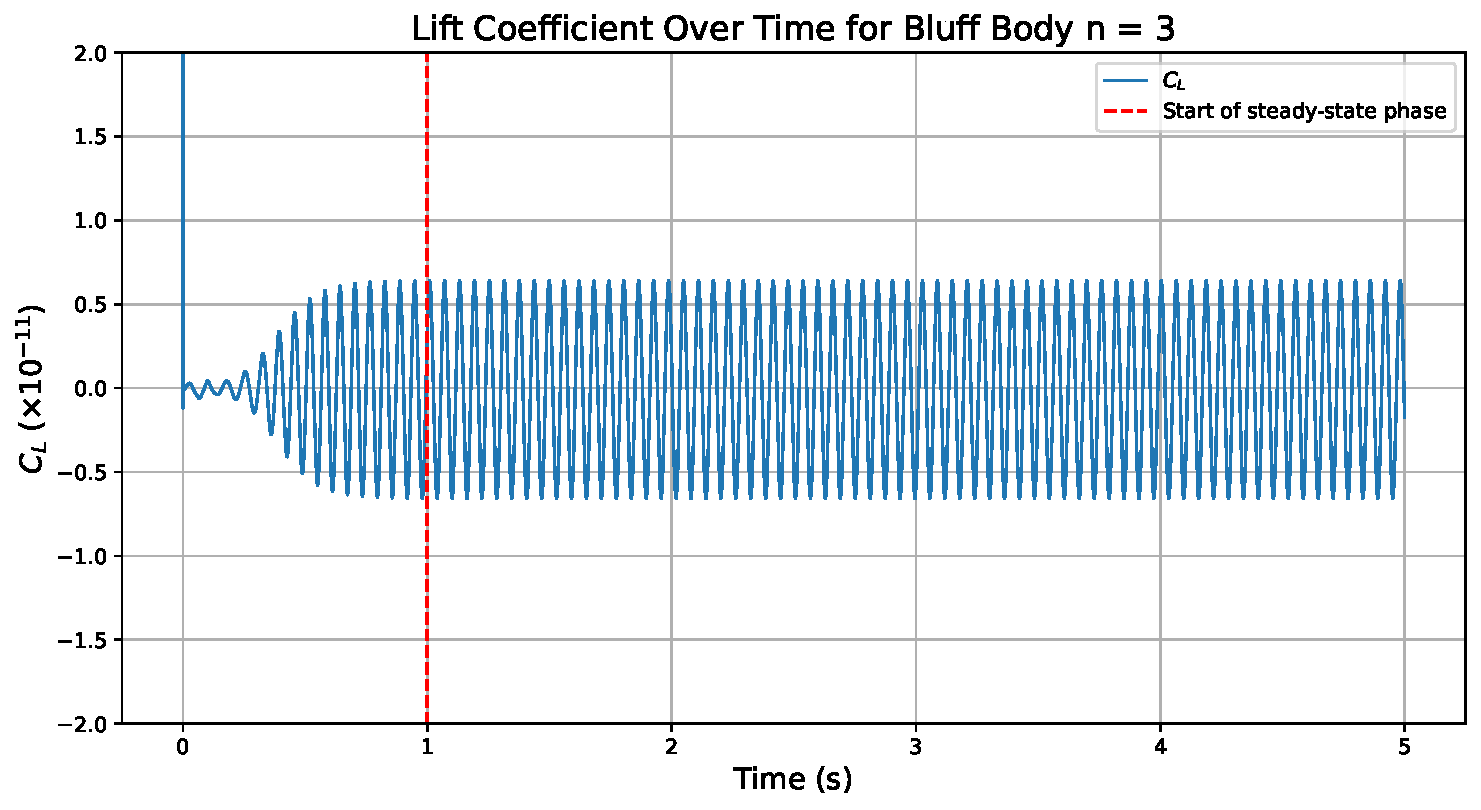
\includegraphics[width=\textwidth]{images/3face_graph}
	\caption{Lift coefficient $C_L$ over time for the bluff body $n=3$. The red dashed line indicates the start of periodic vortex shedding at $t = 1\,\mathrm{s}$.}
	\label{fig:3FaceGraph} 
\end{figure}

\begin{figure}[H]
	\centering
	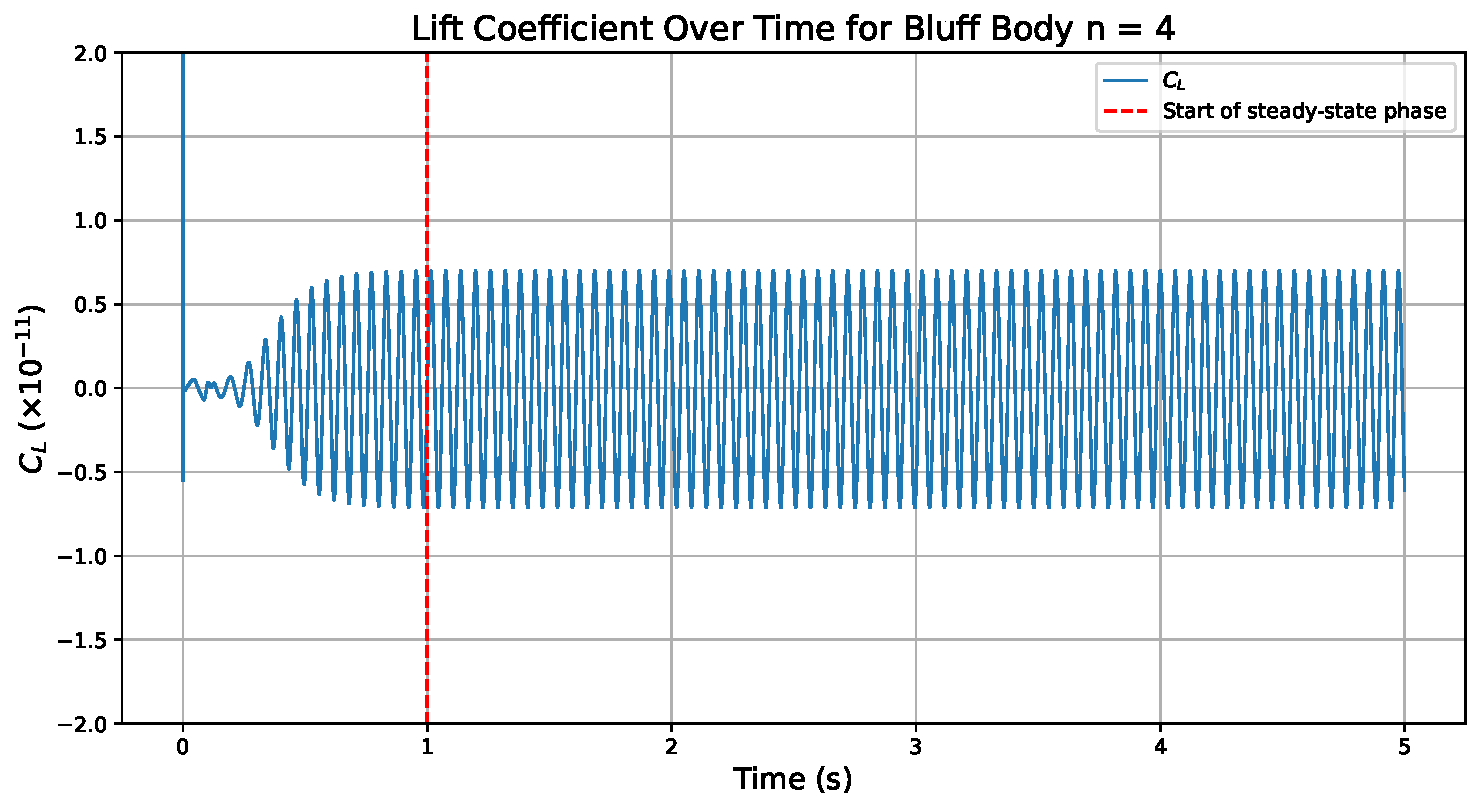
\includegraphics[width=\textwidth]{images/4face_graph}
	\caption{Lift coefficient $C_L$ over time for the bluff body $n=3$. The red dashed line indicates the start of periodic vortex shedding at $t = 1\,\mathrm{s}$.}
	\label{fig:4FaceGraph} 
\end{figure}

\begin{figure}[H]
	\centering
	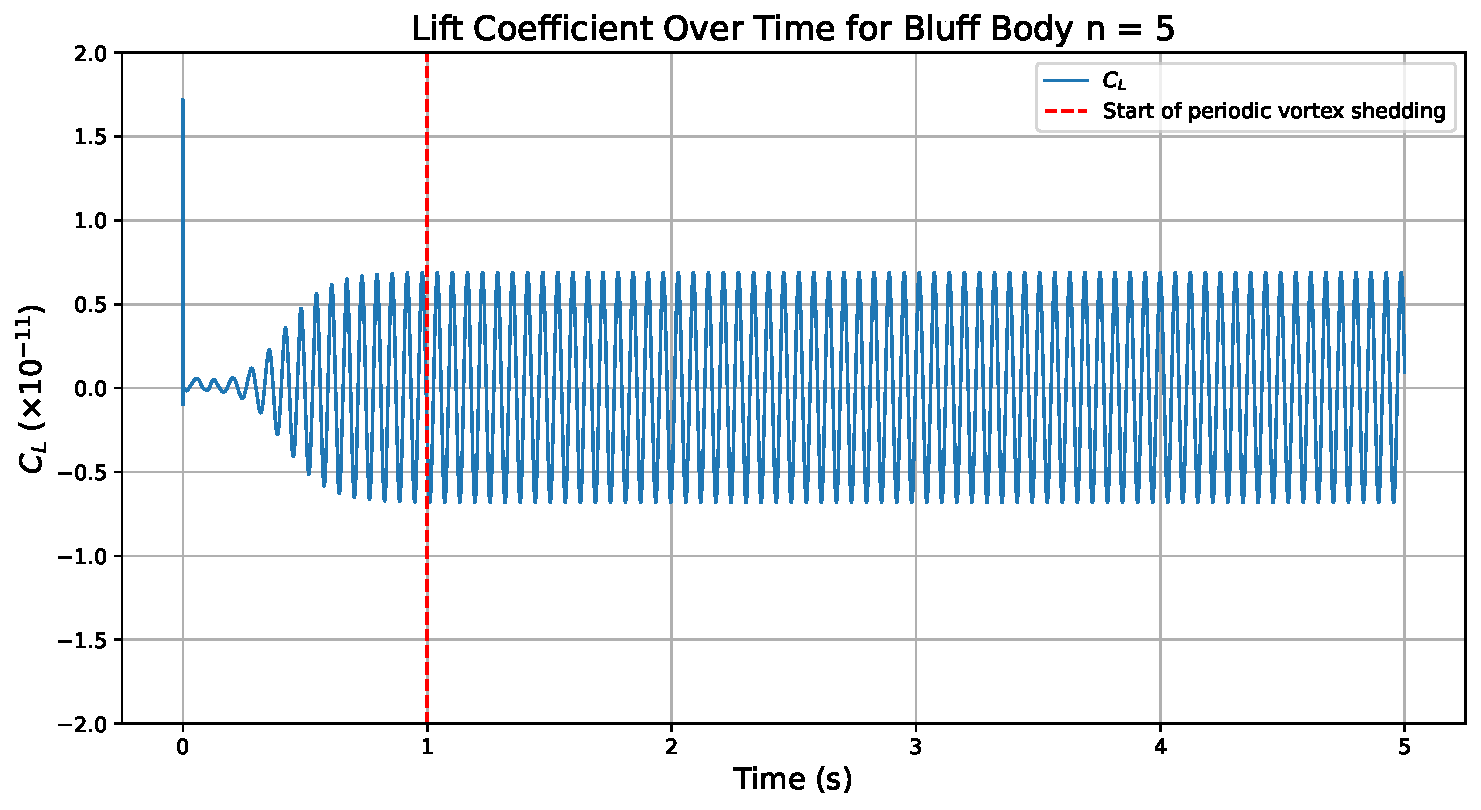
\includegraphics[width=\textwidth]{images/5face_graph}
	\caption{Lift coefficient $C_L$ over time for the bluff body $n=3$. The red dashed line indicates the start of periodic vortex shedding at $t = 1\,\mathrm{s}$.}
	\label{fig:5FaceGraph} 
\end{figure}

\begin{figure}[H]
	\centering
	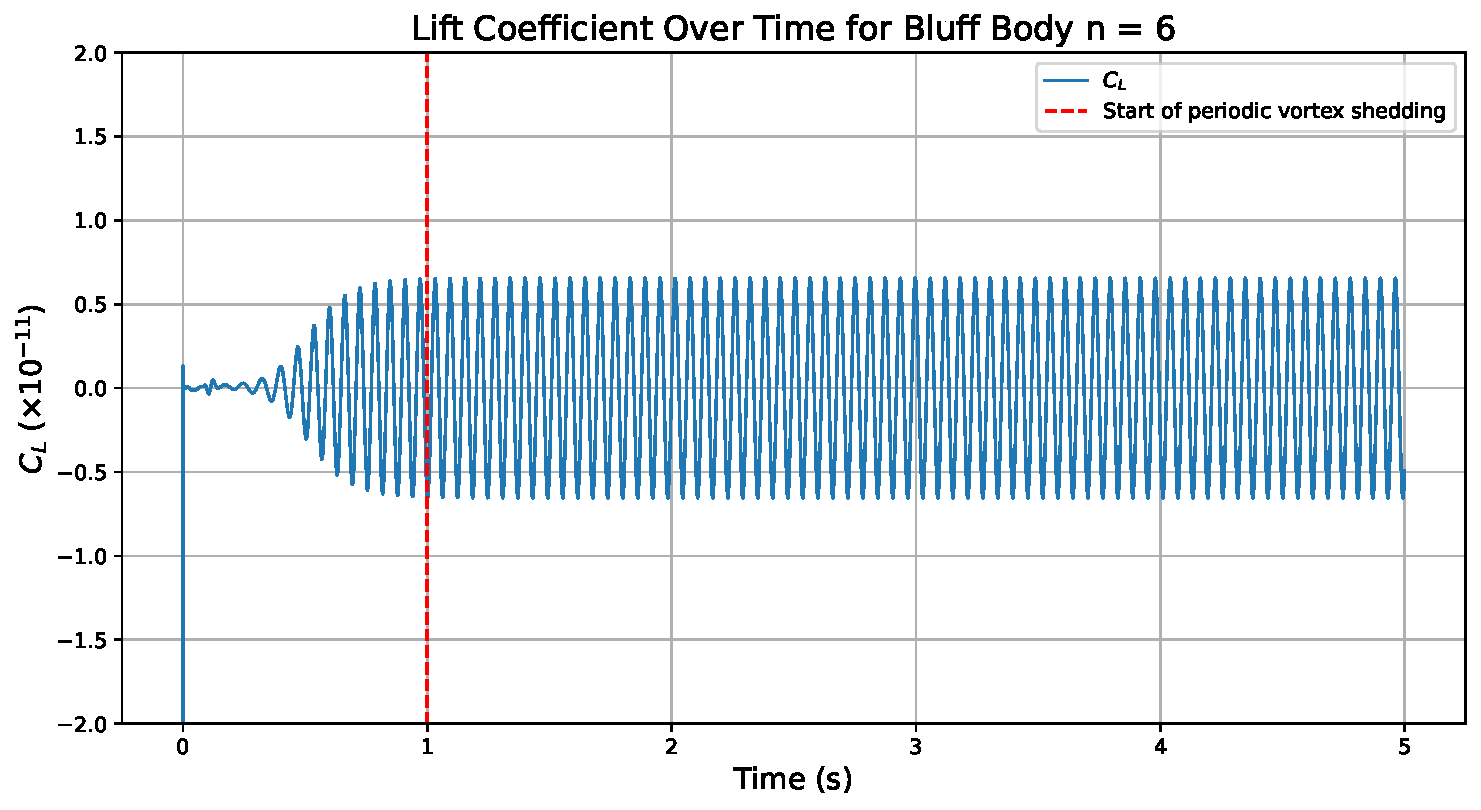
\includegraphics[width=\textwidth]{images/6face_graph}
	\caption{Lift coefficient $C_L$ over time for the bluff body $n=3$. The red dashed line indicates the start of periodic vortex shedding at $t = 1\,\mathrm{s}$.}
	\label{fig:6FaceGraph} 
\end{figure}

\begin{figure}[H]
	\centering
	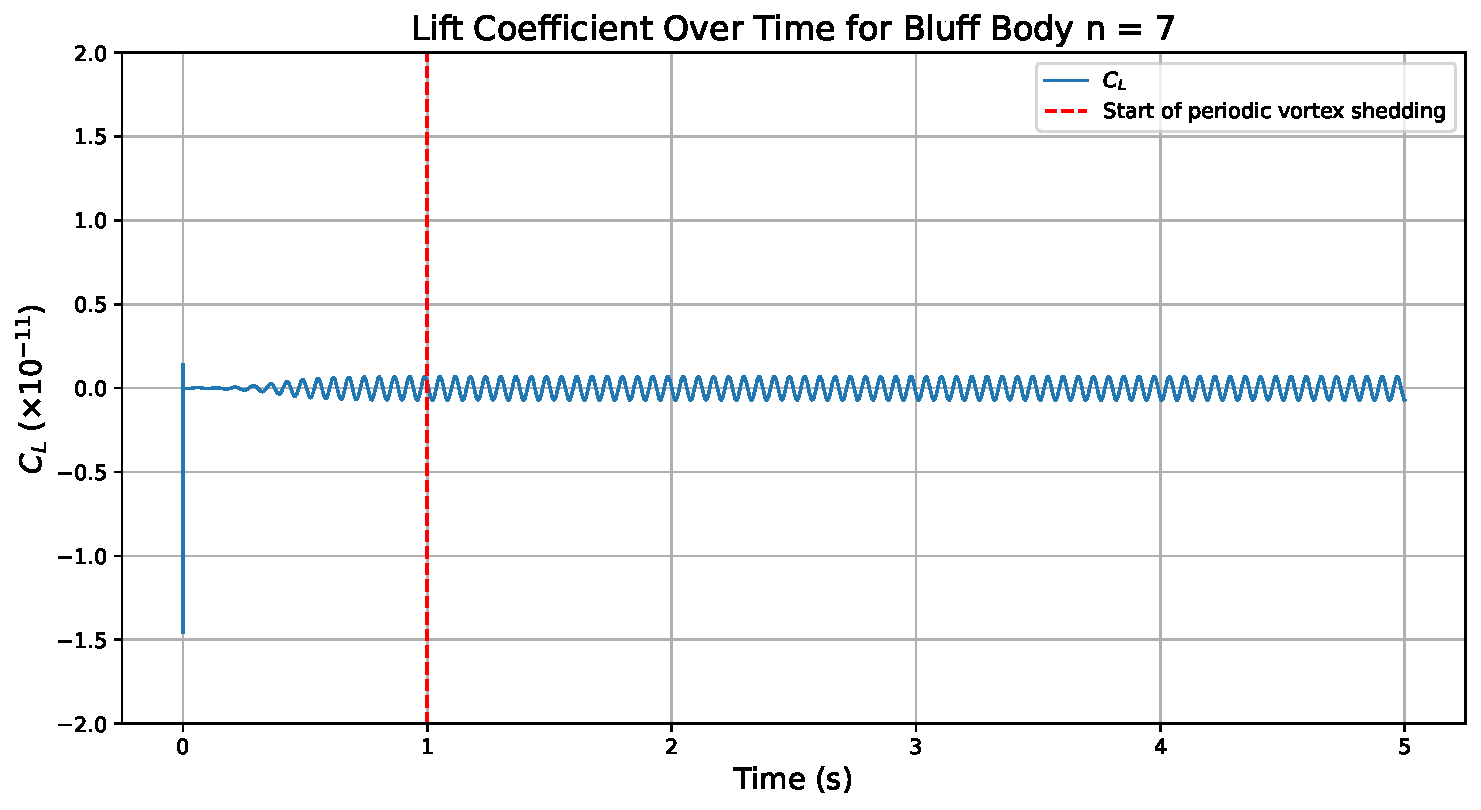
\includegraphics[width=\textwidth]{images/7face_graph}
	\caption{Lift coefficient $C_L$ over time for the bluff body $n=3$. The red dashed line indicates the start of periodic vortex shedding at $t = 1\,\mathrm{s}$.}
	\label{fig:7FaceGraph} 
\end{figure}

\begin{figure}[H]
	\centering
	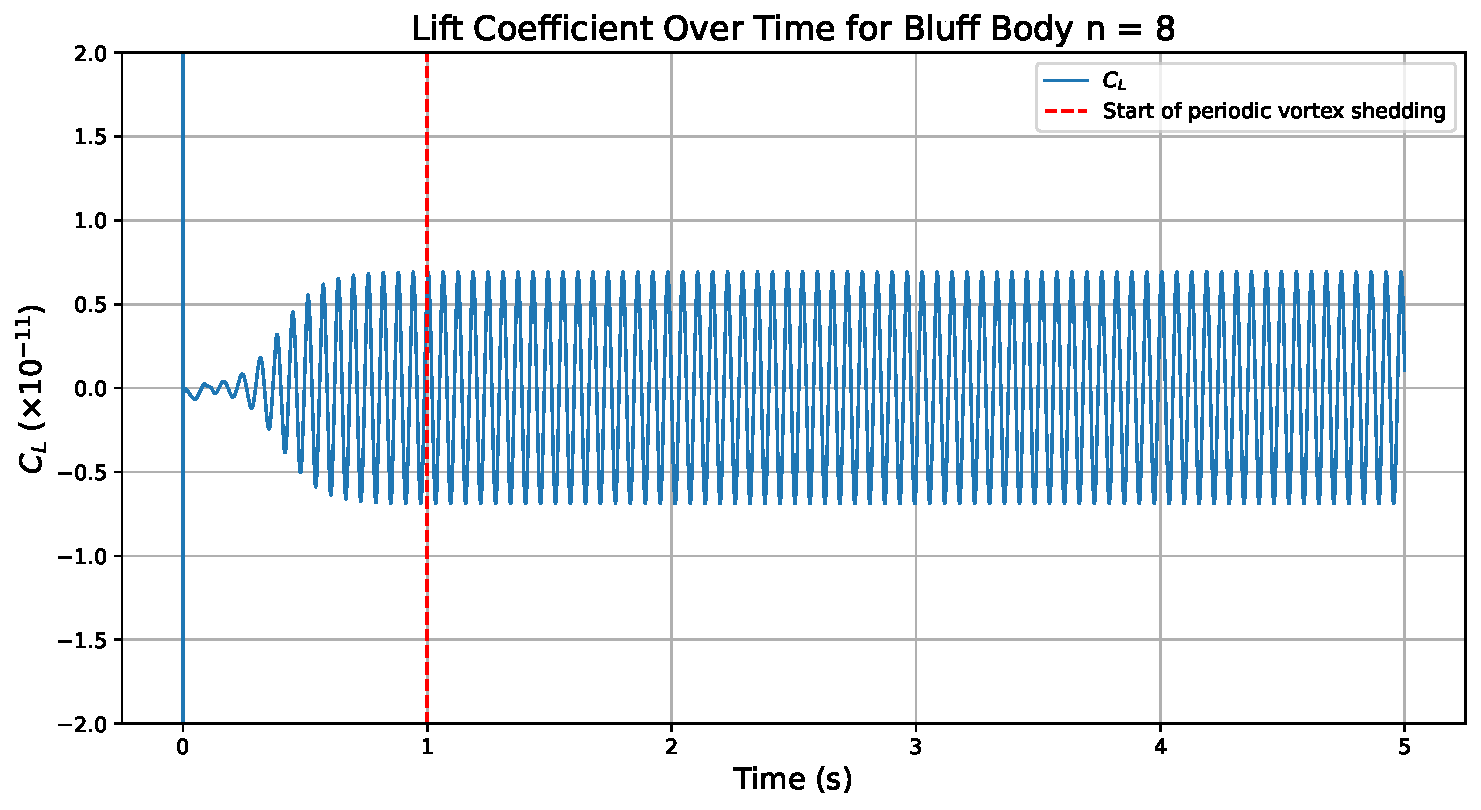
\includegraphics[width=\textwidth]{images/8face_graph}
	\caption{Lift coefficient $C_L$ over time for the bluff body $n=3$. The red dashed line indicates the start of periodic vortex shedding at $t = 1\,\mathrm{s}$.}
	\label{fig:8FaceGraph} 
\end{figure}

\begin{figure}[H]
	\centering
	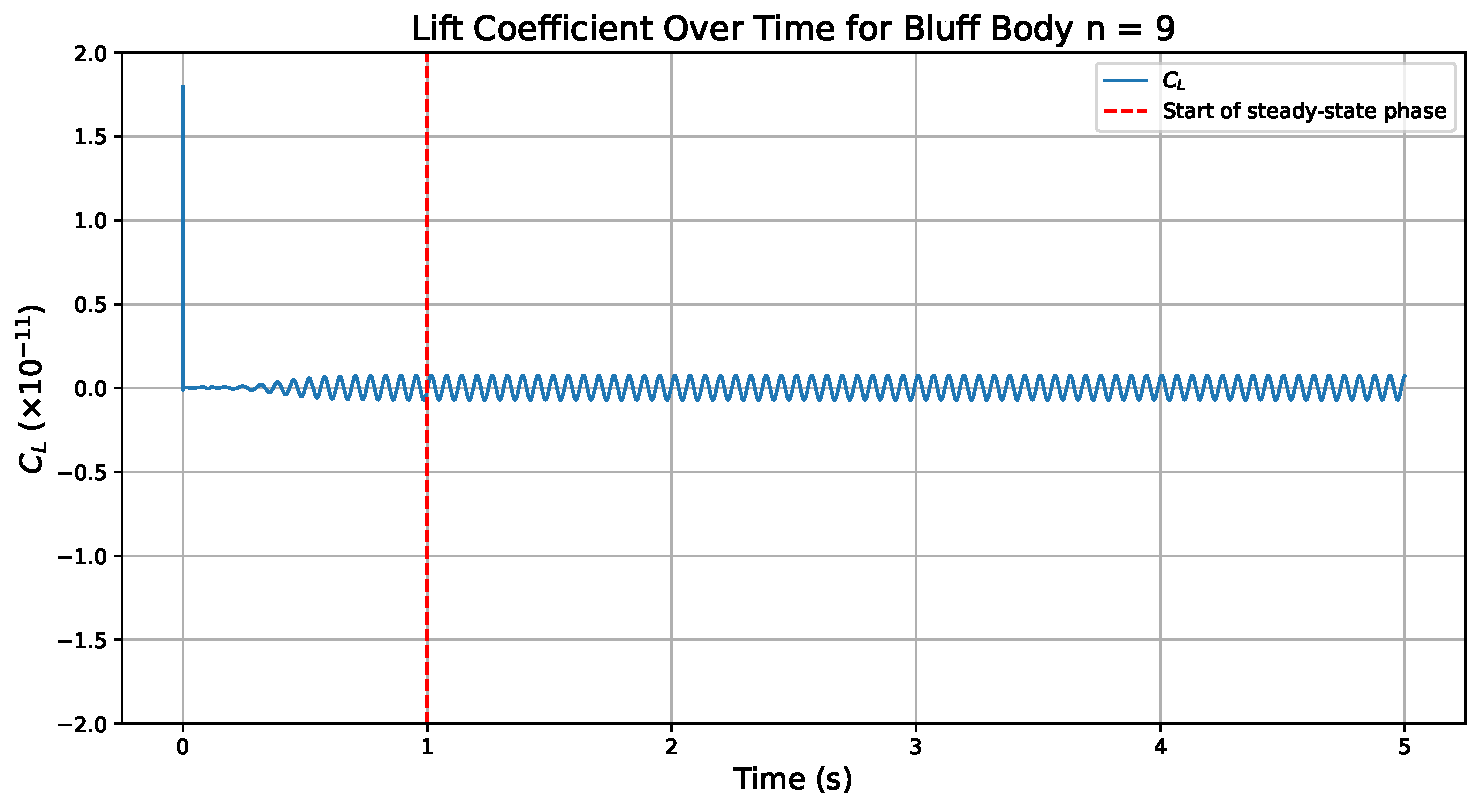
\includegraphics[width=\textwidth]{images/9face_graph}
	\caption{Lift coefficient $C_L$ over time for the bluff body $n=3$. The red dashed line indicates the start of periodic vortex shedding at $t = 1\,\mathrm{s}$.}
	\label{fig:9FaceGraph} 
\end{figure}

\begin{figure}[H]
	\centering
	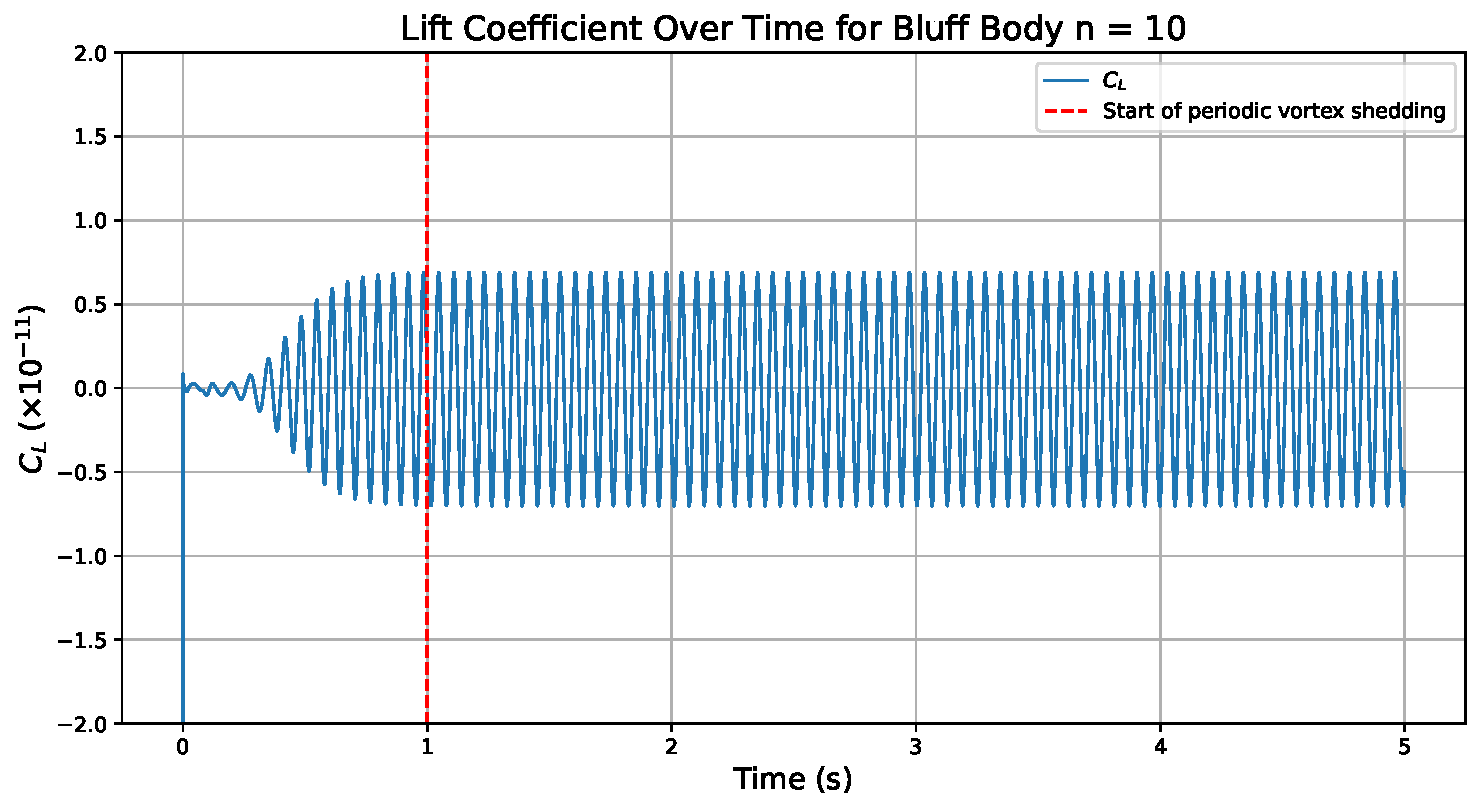
\includegraphics[width=\textwidth]{images/10face_graph}
	\caption{Lift coefficient $C_L$ over time for the bluff body $n=3$. The red dashed line indicates the start of periodic vortex shedding at $t = 1\,\mathrm{s}$.}
	\label{fig:10FaceGraph} 
\end{figure}

\begin{figure}[H]
	\centering
	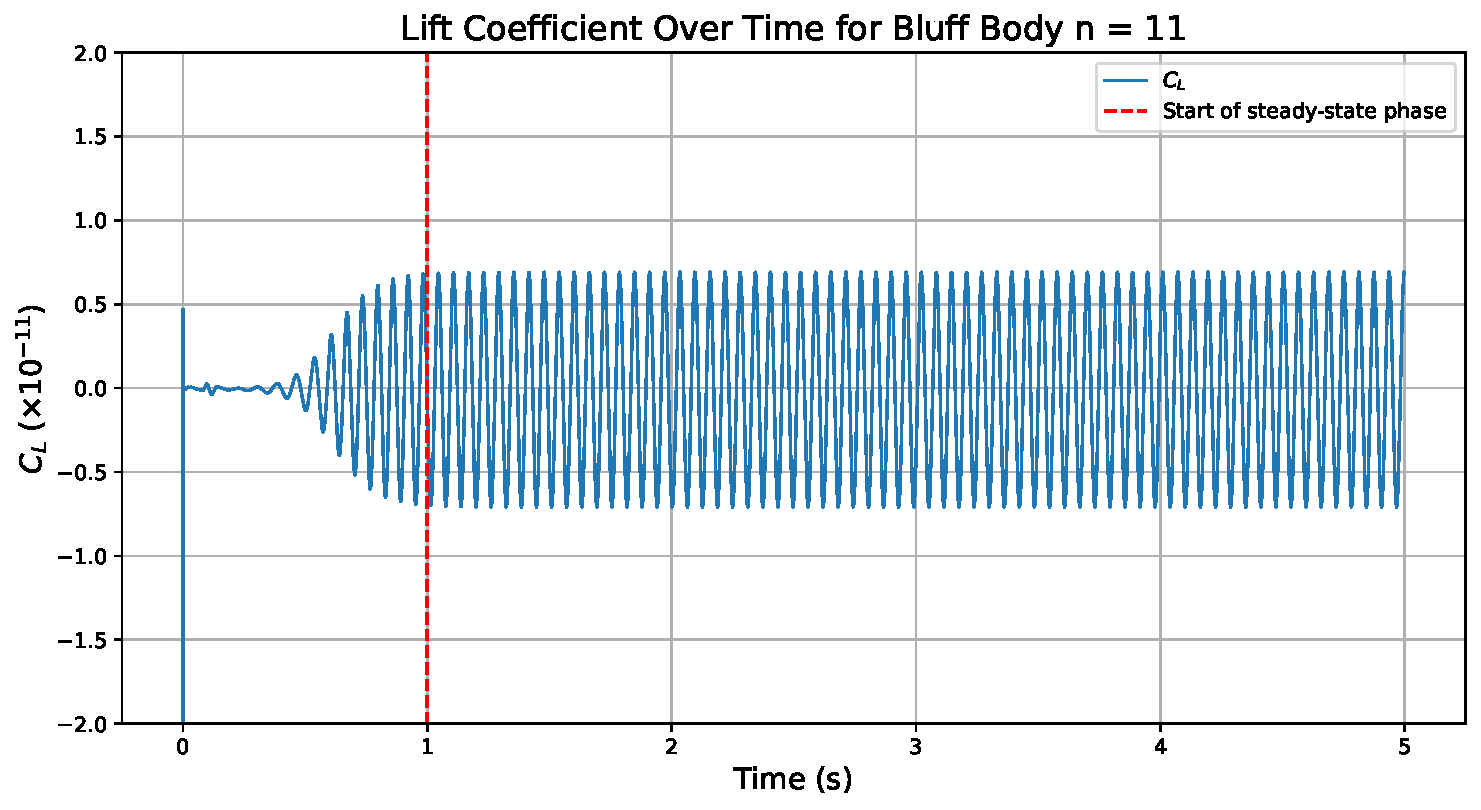
\includegraphics[width=\textwidth]{images/11face_graph}
	\caption{Lift coefficient $C_L$ over time for the bluff body $n=3$. The red dashed line indicates the start of periodic vortex shedding at $t = 1\,\mathrm{s}$.}
	\label{fig:11FaceGraph} 
\end{figure}

\begin{figure}[H]
	\centering
	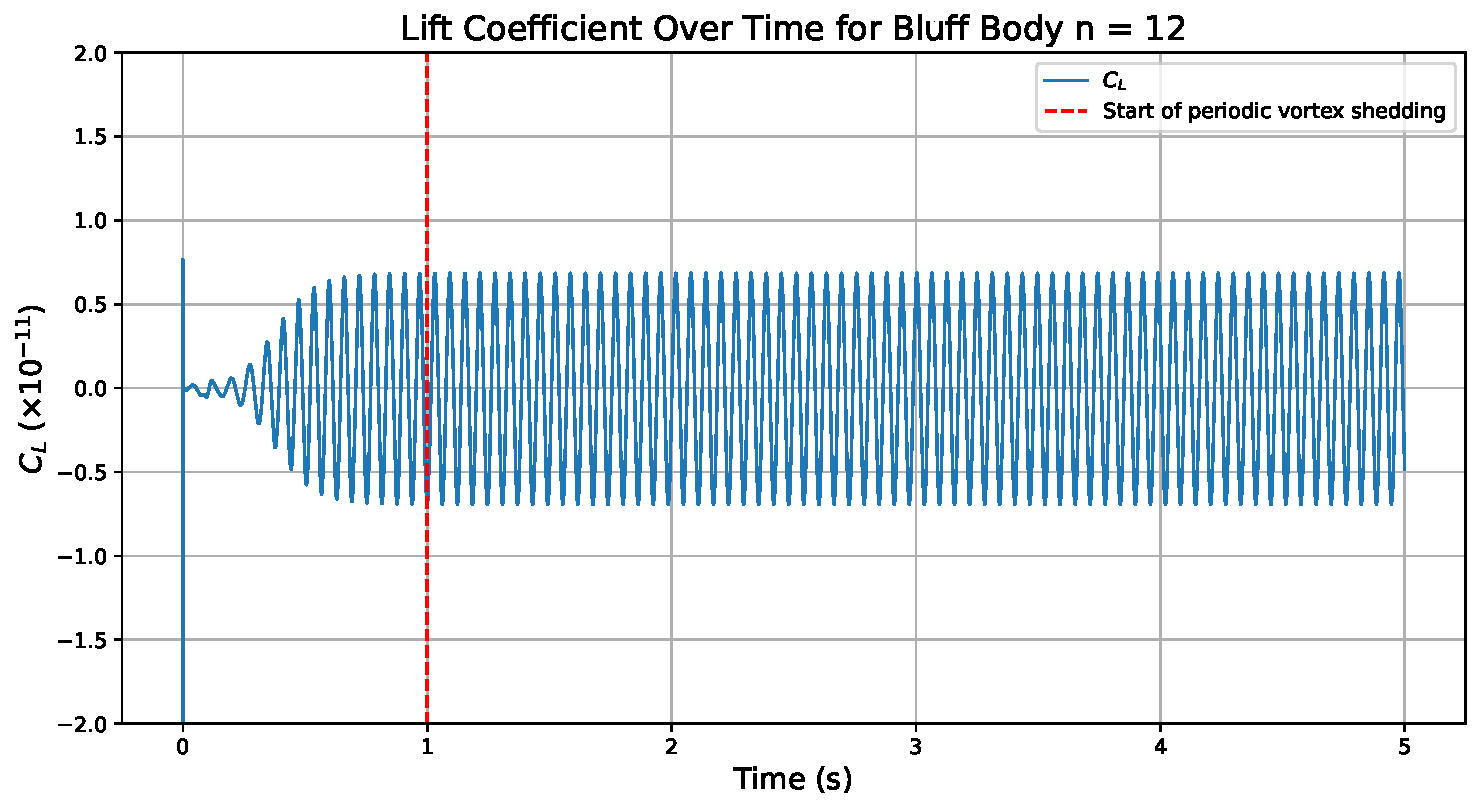
\includegraphics[width=\textwidth]{images/12face_graph}
	\caption{Lift coefficient $C_L$ over time for the bluff body $n=3$. The red dashed line indicates the start of periodic vortex shedding at $t = 1\,\mathrm{s}$.}
	\label{fig:12FaceGraph} 
\end{figure}

\subsubsection{Sample Calculation of Vortex Shedding Frequency for Bluff Body $n=2$ using Python}

\begin{figure}[H]
	\centering
	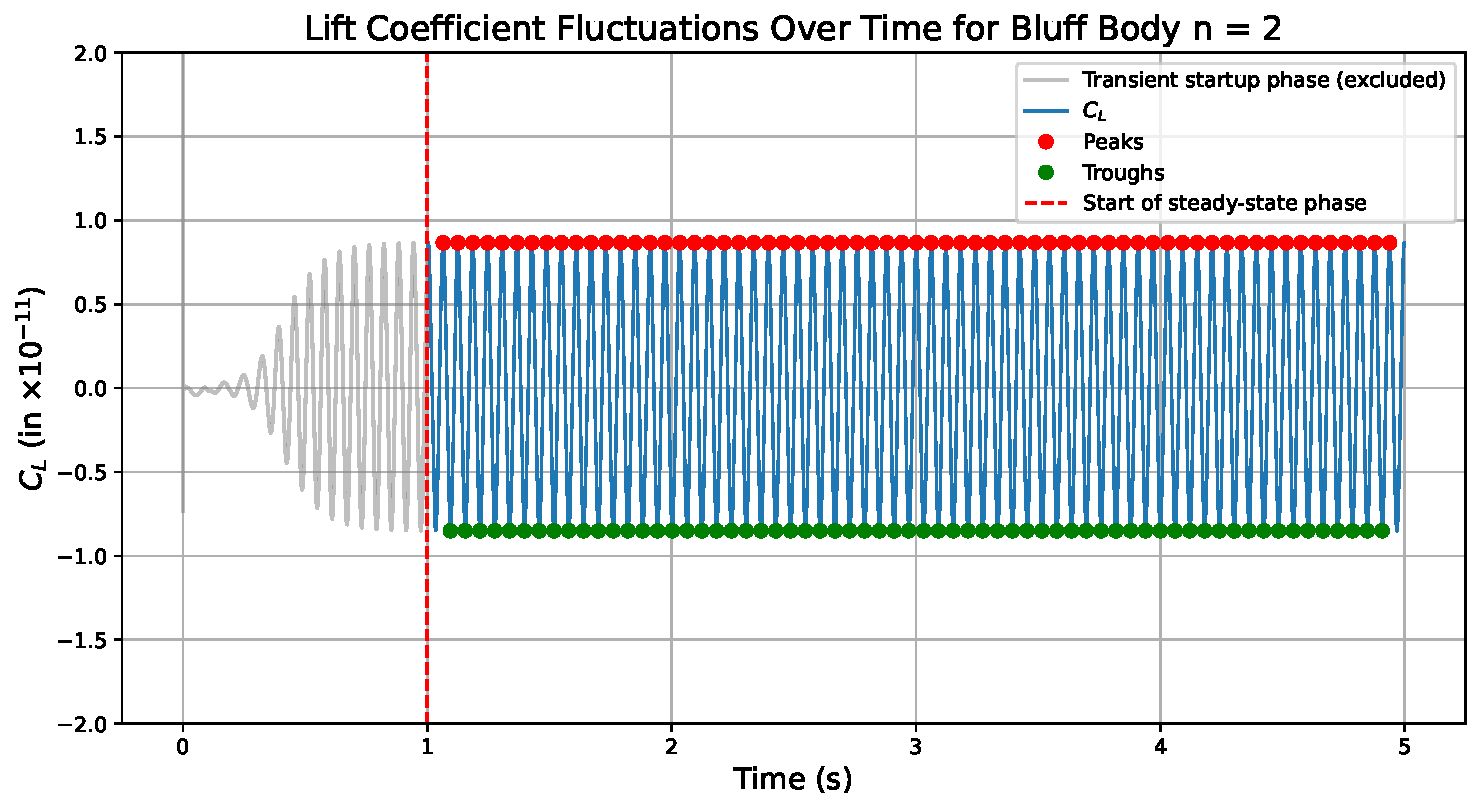
\includegraphics[width=\textwidth]{images/2face_graph_sample_Calc}
	\caption{Sample visualization of the peaks and troughs identification on the Lift Coefficient $C_L$ over time graph for bluff body $n=2$. The initial startup phase, colored in gray, is excluded from the detection.}
	\label{fig:2FaceGraphSampleCalc} 
\end{figure}

\begin{tcolorbox}[title=Python Output,fonttitle=\bfseries,
	colframe=black!75!white,colback=gray!10!white,boxrule=0.5pt,
	fontupper=\ttfamily]
	Number of peaks:    65 \\
	Number of troughs:  64 \\
	
	Average time period: 0.06052 s \\
\end{tcolorbox}

Using the outputted average period \( T = 0.06052 \, \text{s} \), the vortex shedding frequency was calculated:

\[
f = \frac{1}{T} = \frac{1}{0.06052} = 16.52346 \, Hz
\]

This represents the vortex shedding frequency of the bluff body with \( n = 2 \) faces in laminar flow.

\subsubsection{A Comparison of Vortex Shedding Frequency with Increasing $n$ from 2 \textendash\ 12}

\begin{table}[H]
	\centering
	\renewcommand{\arraystretch}{1.3}
	\begin{tabular}{|c|c|}
		\hline
		\textbf{Bluff Body $n$} & \textbf{Frequency ($Hz$)} \\
		\hline
		$2$  & $16.52346$ \\
		\hline
		$3$  & $16.36393$ \\
		\hline
		$4$  & $16.41497$ \\
		\hline
		$5$  & $16.22323$ \\
		\hline
		$6$  & $16.28664$ \\
		\hline
		$7$  & $16.07976$ \\
		\hline
		$8$  & $16.32387$ \\
		\hline
		$9$  & $16.05910$ \\
		\hline
		$10$ & $16.09528$ \\
		\hline
		$11$ & $16.18909$ \\
		\hline
		$12$ & $16.21797$ \\
		\hline
	\end{tabular}
	\caption{Vortex shedding frequencies for bluff bodies with $n$ streamwise faces.}
	\label{tab:frequencyData}
\end{table}


\begin{figure}[H]
	\centering
	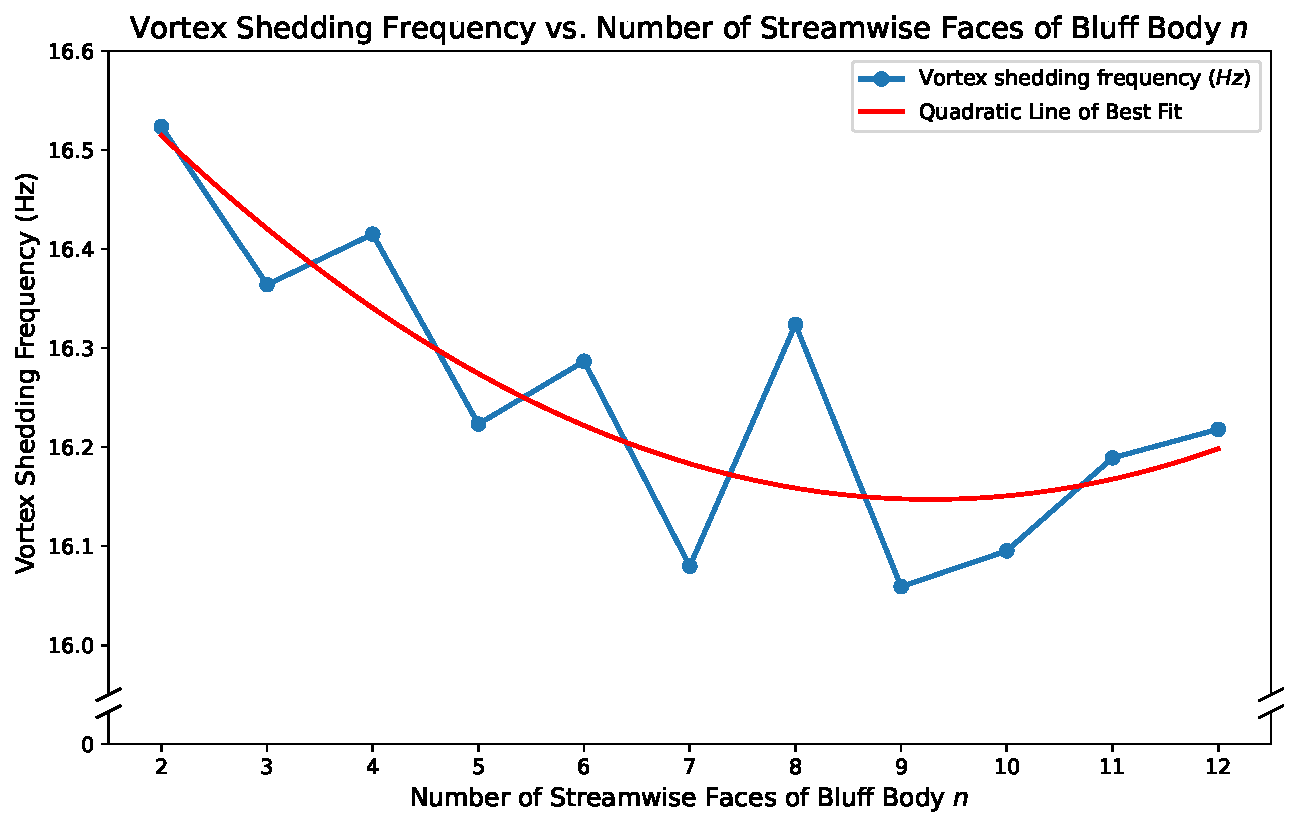
\includegraphics[width=\textwidth]{images/overall}
	\caption{A comparison of vortex shedding frequency with increasing $n$ from 2 \textendash\ 12}
	\label{fig:overall} 
\end{figure}

In order to better visualize the general non-linear trend a quadratic line of best fit was included. 


\subsection{Results of Practical Investigation}
\label{sec:resultsPractical}
The found average flow velocity was $0.04\, m\,s^{-1}$. Despite many attempts to achieve laminar flow, the flow remained turbulent, as demonstrated by the irregular wake patterns and a calculated Reynolds number of 800 \textemdash\ determined using Equation \eqref{eq:reynoldsNumber} where $U = 0.04\,m\,s^{-1}$, $\nu = 1 \times 10^6\, m^2\, s^{-1}$ and $L = 0.02\, m$. Nevertheless, the practical experiment yielded qualitative value. The use of potassium permanganate crystals allowed for a clear visualization of the boundary layer, flow separation and vortex shedding for different bluff bodies.


	
\foreach \n in {2,...,12} {
	\subsubsection*{Snapshots of the Practical Run of Bluff Body $n = \n$}
	\begin{figure}[H]
		\centering
		
		% === Row 1 ===
		\begin{subfigure}[t]{0.48\textwidth}
			\centering
			\includegraphics[width=\linewidth]{images/\n Face/\n Face_0s.jpg}
			\caption{Snapshot of bluff body $n = \n$ at time 0 seconds}
		\end{subfigure}
		\hfill
		\begin{subfigure}[t]{0.48\textwidth}
			\centering
			\includegraphics[width=\linewidth]{images/\n Face/\n Face_1s.jpg}
			\caption{Snapshot of bluff body $n = \n$ at time 1 second}
		\end{subfigure}
		
		\vspace{1em}
		
		% === Row 2 ===
		\begin{subfigure}[t]{0.48\textwidth}
			\centering
			\includegraphics[width=\linewidth]{images/\n Face/\n Face_2s.jpg}
			\caption{Snapshot of bluff body $n = \n$ at time 2 seconds}
		\end{subfigure}
		\hfill
		\begin{subfigure}[t]{0.48\textwidth}
			\centering
			\includegraphics[width=\linewidth]{images/\n Face/\n Face_3s.jpg}
			\caption{Snapshot of bluff body $n = \n$ at time 3 seconds}
		\end{subfigure}
		
		\vspace{1em}
		
		% === Row 3 ===
		\begin{subfigure}[t]{0.48\textwidth}
			\centering
			\includegraphics[width=\linewidth]{images/\n Face/\n Face_4s.jpg}
			\caption{Snapshot of bluff body $n = \n$ at time 4 seconds}
		\end{subfigure}
		\hfill
		\begin{subfigure}[t]{0.48\textwidth}
			\centering
			\includegraphics[width=\linewidth]{images/\n Face/\n Face_5s.jpg}
			\caption{Snapshot of bluff body $n = \n$ at time 5 seconds}
		\end{subfigure}
		
	\end{figure}
}


	
	
	
	




